\begin{figure}[h!]
	\centering
	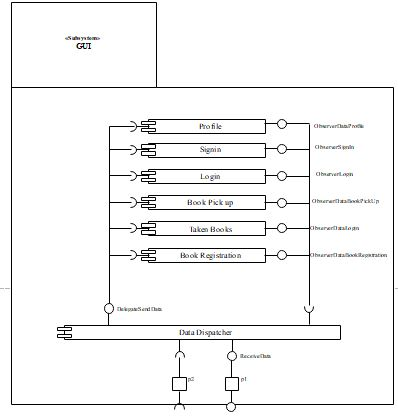
\includegraphics[width=0.8\textwidth]{Immagini/GUI_subsys}
	\caption{Logical view - GUI subsystem}
	\label{fig:LogicalView_GUIsubsys}
\end{figure}
\begin{figure}[h!]
	\centering
	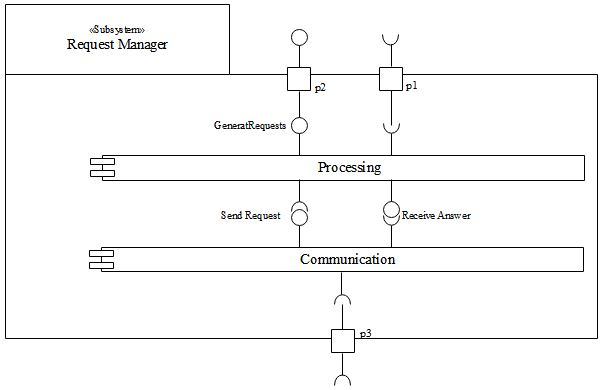
\includegraphics[width=0.8\textwidth]{Immagini/RequestManager_subsys}
	\caption{Logical view - Request Manager subsystem}
	\label{fig:LogicalView_RMsubsys}
\end{figure}
\begin{figure}[h!]
	\centering
	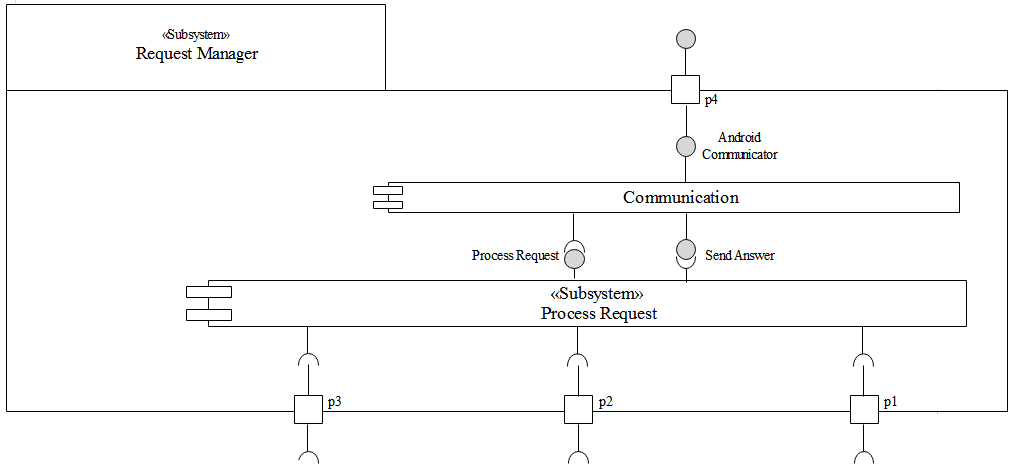
\includegraphics[width=0.8\textwidth]{Immagini/RequestManagerSrv_subsys}
	\caption{Logical view - Request Manager subsystem server side}
	\label{fig:LogicalView_RM_server_subsys}
\end{figure}
\begin{figure}[h!]
	\centering
	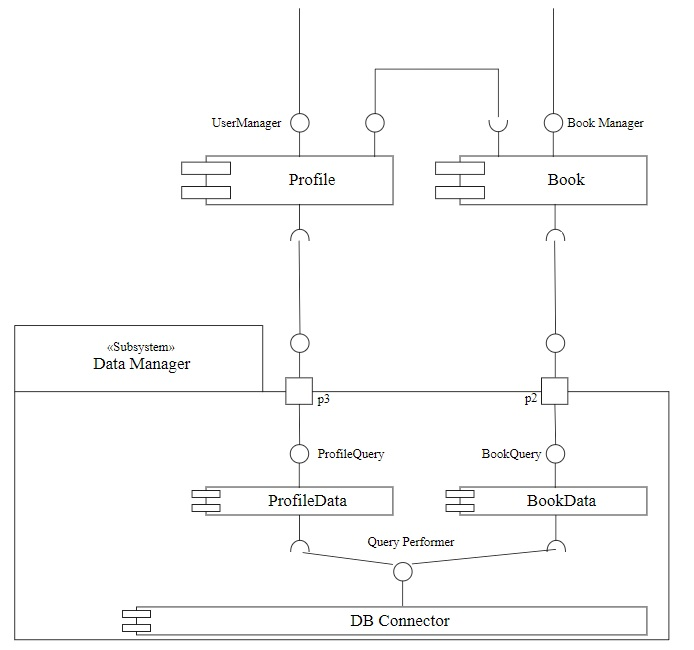
\includegraphics[width=0.8\textwidth]{Immagini/Server_subsys}
	\caption{Logical view - Server functionality}
	\label{fig:LogicalView_ServerSubsys}
\end{figure}
\noindent
Nelle figure ~\ref{fig:LogicalView_GUIsubsys}, ~\ref{fig:LogicalView_RMsubsys}, ~\ref{fig:LogicalView_RM_server_subsys} e ~\ref{fig:LogicalView_ServerSubsys} è mostrata in dettaglio la Logical View del sistema progettato. Si può osservare che segue il modello definito attraverso il pattern archietteturale Model View Controller, dal momento che vengono individuati tre strati, ciascuno dei quali con le seguenti caratteristiche:
\begin{itemize}
	\item\label{subsysGUI} \textbf{Subsystem \textit{"GUI”:}} rappresenta l’interfaccia grafica con la quale l’applicazione si presenterà. Ciascun componente fa riferimento ad ogni view che l'applicazione può mnostrare, e che quindi corrisponde a diffenti casi d'uso dell'applicativo stesso, come l’accesso alla rete di Book Crossing (Login) o registrazione di un  libro.
	
	Questi componenti saranno quindi ovviamente allocati direttamente sul dispositivo mobile: ogni singolo component (\textit{fragment}) avrà legato ad esso, in maniera intrinseca, anche un file \textit{.xml}, il quale permette di definirne l'interfaccia grafica, ovvero come sono posizionati gli elementi visivi.
	
	TODO: spiegazione sintetica delle funzionalità di ogni singolo fragment
	
	\item\label{subsysRequestManager} \textbf{Subsystem \textit{"Request Manager”:}} ha il compito di gestire le richieste provenienti da ciascun componente descritto nel subsystem \textit{GUI”}. Al suo interno sono indicati i componenti attraverso i quali si risponde alle richieste provenienti dal dispositivo mobile.
	
	Una parte di questo \textit{manager} sarà disposta a bordo del dispositivo, permettendo una preelaborazione e assemblamento delle richieste; questo subsystem avrà però anche un implementazione \textit{server side}, che gli permetterà di ricevere tali richieste, rieditarla, secondo quello che è la necessità della richiesta, e poi interacciarsi, in un verso o nell'altro, con la parte di persistenza dei dati.
	\item\label{subsysDataManager} \textbf{Subsystem \textit{"Data Manager":}} ”: rappresenta la comunicazione con il Database. Sono quindi indicati i componenti con i quali il sistema si interfaccerà con la banca dati dell’architettura.
\end{itemize}

Si vede quindi come ogni parte dell'archietettura abbia un compito ben definito: la parte relativa al subsystem \textit{GUI (Graphic User Interface)}, si occupa di gestire l'interazione con l'utente ricevendo e/o mostrando i dati forniti e/o richieste dall'utilizzatore stesso; al suo interno quindi non trovermo codice di logica applicativa ma solamente componenti di gestione \textit{UI}. Esso rappresenta quindi la parte di \textit{\textbf{view}}.
Il subsystem \textit{request manager} invece si occupa di controllare il flusso di dati dall'applicazione al server e viceversa; rappresenta quindi la sezione di \textit{\textbf{controller}} dove è contenuta la \textit{low logic} dell'applicazione.
Infine, il terzo ed ultimo componente della struttura MVC, è rappresentato dal subsystem \textit{data manager}, il quale permette di interfacciarsi direttamente con la base di dati, astrendo tutte le operazione di controllo di accesso al database stesso.
Il modello architetturale MVC è stato poi applicato anche successivamente per la progettazione delle componenti previste per ciascun elemento dell'architettura.